\subsection{pbdMPI Example: Monte Carlo Simulation}
\makesubcontentsslidessec


\begin{frame}
  \begin{block}{Example \countex :  Monte Carlo Simulation}\pause
  Sample $N$ uniform observations $(x_i, y_i)$ in the unit square $[0, 1]\times [0,1]$.  Then
\begin{equation*}
\pi \approx 4\left(\frac{\#\ Inside\ Circle}{\#\ Total}\right) = 4\left(\frac{\text{\color{blue}{\# 
Blue}}}{\text{\color{blue}{\# Blue}}+\text{\color{red}{\# Red}}}\right)
\label{eqn:pi}
\end{equation*}
  \begin{center}
   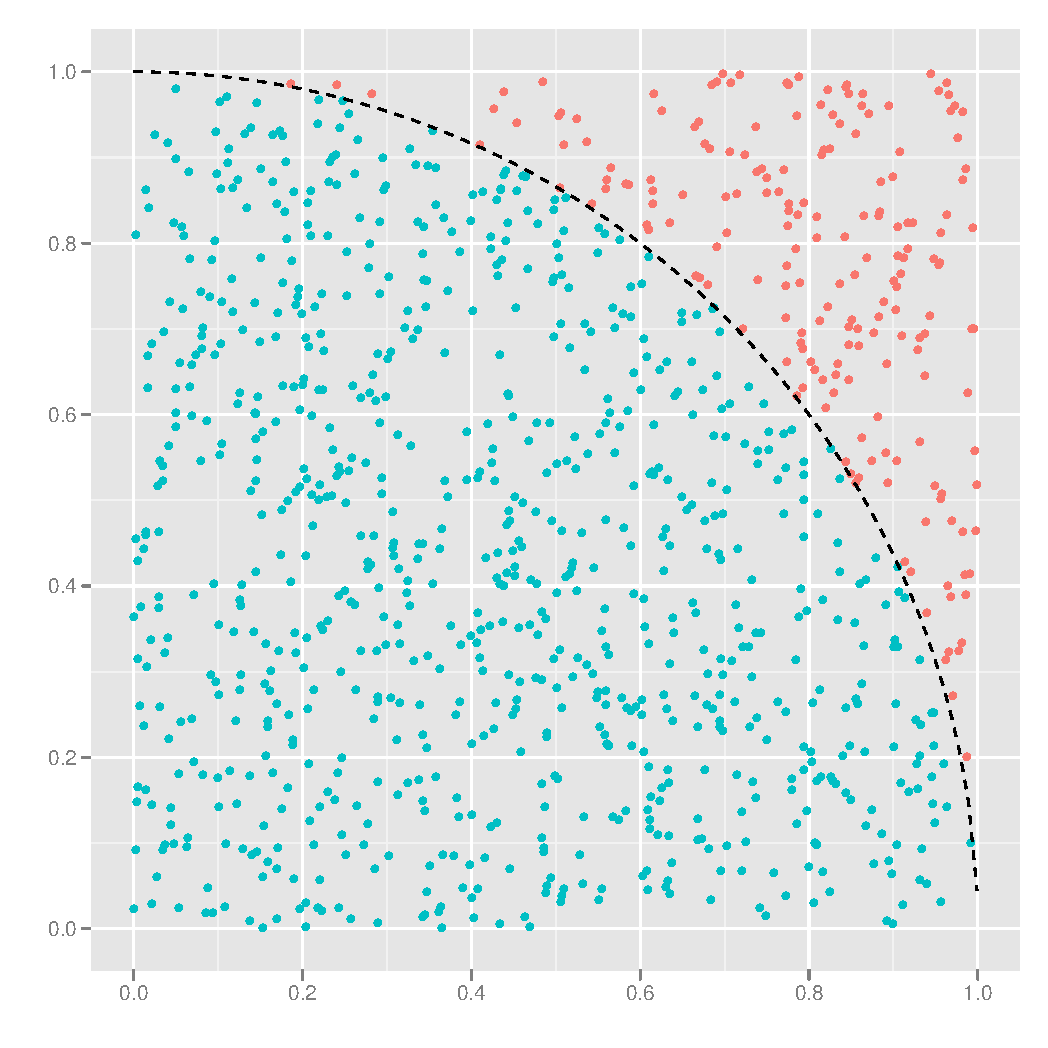
\includegraphics[scale=.25]{../common/pics/pi} 
  \end{center}
  \end{block}
\end{frame}


\begin{frame}[fragile]
  \begin{block}{Example \showex :  Monte Carlo Simulation GBD Algorithm}\pause
    \begin{enumerate}
     \item Let $n$ be big-ish; we'll take $n=50,000$.
     \item Generate an $n\times 2$ matrix $x$ of standard uniform observations.
     \item Count the number of rows satisfying $x^2 + y^2 \leq 1$
     \item Ask everyone else what their answer is; sum it all up.
     \item Take this new answer, multiply by 4 and divide by $n$
     \item If my rank is 0, print the result.
    \end{enumerate}
  \end{block}
\end{frame}


\begin{frame}[fragile,scale,shrink]
  \begin{exampleblock}{Example \showex :  Monte Carlo Simulation Code}\pause
\begin{lstlisting}[title=Serial Code]
N <- 50000
X <- matrix(runif(N * 2), ncol=2)
r <- sum(rowSums(X^2) <= 1)
PI <- 4*r/N
print(PI)
\end{lstlisting}

\begin{lstlisting}[title=Parallel Code]
library(pbdMPI, quiet = TRUE)
init()
comm.set.seed(seed=1234567, diff=TRUE)

N.gbd <- 50000 / comm.size()
X.gbd <- matrix(runif(N.gbd * 2), ncol = 2)
r.gbd <- sum(rowSums(X.gbd^2) <= 1)
r <- allreduce(r.gbd)
PI <- 4*r/(N.gbd * comm.size())
comm.print(PI)

finalize()
\end{lstlisting}
  \end{exampleblock}
\end{frame}

\begin{frame}[fragile]
  \begin{block}{Note}\pause
    For the remainder, we will exclude loading, init, and finalize calls.
  \end{block}
\end{frame}



